\documentclass[tikz,border=10pt]{standalone}
\usepackage{tikz}
\usetikzlibrary{arrows.meta, decorations.pathmorphing, positioning}
\usetikzlibrary{calc}

\newcommand{\styledEllipse}[5]{%
  % left half: from top (90°) down to bottom (270°)
  \draw[#4]
    ($(#1)+(0,#3)$)
    arc[
      x radius=#2,
      y radius=#3,
      start angle=90,
      end angle=270
    ];%
  % right half: from bottom (–90°) up to top (90°)
  \draw[#5]
    ($(#1)+(0,-#3)$)
    arc[
      x radius=#2,
      y radius=#3,
      start angle=-90,
      end angle=90
    ];%
}


\begin{document}
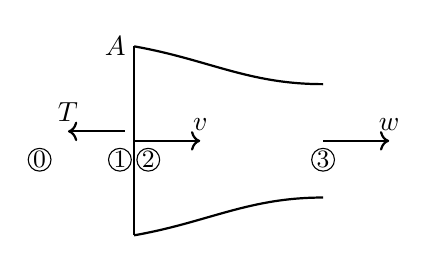
\begin{tikzpicture}[scale=1.2]

\def\length{2cm}

% outer tube
\draw[thick] (0,1) to[out=-10,in=180] (\length,0.6);
\draw[thick] (0,-1)  to[out=10,in=180] (\length,-0.6) ;
\draw[thick] (0, -1) -- (0, 1);


\draw[thick,->] (0,0) -- (0.7,0) node[above] {$v$};
\draw[thick,->] (\length,0) -- (\length + 0.7cm,0) node[above] {$w$};

\draw[thick,->] (-0.1,0.1) -- (-0.7,0.1) node[above] {$T$};

\node at (-0.2, 1) {$A$};

\foreach \label/\x in {0/-1,1/-0.15,2/0.15,3/\length} {
    \node[
      draw,
      circle,
      inner sep=0.3pt,      % smaller padding
      font=\small,           % tiny font size
      fill=white            % optional: cover the line underneath
    ] at (\x,-0.2) {\label};
  }


\end{tikzpicture}
\end{document}